%%%%%%%%%%%%%%%%%%%%%%%%%%%%%%%%%%%%%%%%%
% Masters/Doctoral Thesis
% LaTeX Template
% Version 2.1 (2/9/15)
%
% This template has been downloaded from:
% http://www.LaTeXTemplates.com
%
% Version 2.0 major modifications by:
% Vel (vel@latextemplates.com)
%
% Original authors:
% Steven Gunn  (http://users.ecs.soton.ac.uk/srg/softwaretools/document/templates/)
% Sunil Patel (http://www.sunilpatel.co.uk/thesis-template/)
%
% License:
% CC BY-NC-SA 3.0 (http://creativecommons.org/licenses/by-nc-sa/3.0/)
%
%%%%%%%%%%%%%%%%%%%%%%%%%%%%%%%%%%%%%%%%%

%----------------------------------------------------------------------------------------
%	PACKAGES AND OTHER DOCUMENT CONFIGURATIONS
%----------------------------------------------------------------------------------------
%para deixar o arquivo com estilo livro, comentar o "oneside"
\documentclass[
12pt, % The default document font size, options: 10pt, 11pt, 12pt
%oneside, Twoside (alternating margins) for binding by default, uncomment to switch to one side
english, brazil, % ngerman for German
%singlespacing, % Single line spacing, alternatives:
%onehalfspacing,  or
doublespacing,
%draft, % Uncomment to enable draft mode (no pictures, no links, overfull hboxes indicated)
nolistspacing, % If the document is onehalfspacing or doublespacing, uncomment this to set spacing in lists to single
liststotoc, % Uncomment to add the list of figures/tables/etc to the table of contents
%toctotoc, % Uncomment to add the main table of contents to the table of contents
%parskip, % Uncomment to add space between paragraphs
]{MastersDoctoralThesis} % The class file specifying the document structure

\usepackage[utf8]{inputenc} % Required for inputting international characters
\usepackage[T1]{fontenc} % Output font encoding for international characters
%\usepackage[english, brazil]{babel}
%\usepackage{palatino} % Use the Palatino font by default

\usepackage[backend=bibtex,style=authoryear,natbib=true]{biblatex} % User the bibtex backend with the authoryear citation style (which resembles APA)

%\usepackage{scrextend}

\addbibresource{references/ref.bib} % The filename of the bibliography

%\usepackage[authoryear]{natbib}
%\bibliographystyle{apalike}


\usepackage[autostyle=true]{csquotes} % Required to generate language-dependent quotes in the bibliography

\usepackage{mathtools}
\usepackage{verbatim}
\usepackage[]{graphicx}
\usepackage{caption}   %para subfiguras
\usepackage{subcaption}%para subfiguras
\usepackage{float}
\graphicspath{ {figuras/} }
%\graphicspath{{/home/glauffer/Dropbox/FURG/final_project/monografia/figuras}}
\usepackage{color}
\usepackage{siunitx}
\usepackage{indentfirst}

%para numerar subsection e aparecer no toc
\setcounter{secnumdepth}{3}
\setcounter{tocdepth}{3}
\usepackage[linesnumbered, ruled, figure, portuguese]{algorithm2e}
\SetKwBlock{Inicio}{Início}{Fim}
\SetKwFor{ParaCada}{para cada}{faça}{fim para}
\usepackage{listings}

\lstset{
  language=Python,
  showstringspaces=false,
  formfeed=newpage,
  tabsize=4,
  basicstyle=\footnotesize
}



%----------------------------------------------------------------------------------------
%	THESIS INFORMATION
%----------------------------------------------------------------------------------------

\thesistitle{Determinação de Períodos de Pulsação Estelar Através da Entropia Condicional de Shannon} % Your thesis title, this is used in the title and abstract, print it elsewhere with \ttitle
\engthesistitle{Conditional Shannon Entropy Method to Detect Periods on Variable Stars}
\supervisor{ Prof. Dr. Fabricio Ferrari} % Your supervisor's name, this is used in the title page, print it elsewhere with \supname
\examiner{} % Your examiner's name, this is not currently used anywhere in the template, print it elsewhere with \examname
\degree{Bacharel em Física} % Your degree name, this is used in the title page and abstract, print it elsewhere with \degreename
\author{Gabriel Lauffer Ramos} % Your name, this is used in the title page and abstract, print it elsewhere with \authorname
%\addresses{} % Your address, this is not currently used anywhere in the template, print it elsewhere with \addressname

%\subject{Biological Sciences} % Your subject area, this is not currently used anywhere in the template, print it elsewhere with \subjectname
\keywords{} % Keywords for your thesis, this is not currently used anywhere in the template, print it elsewhere with \keywordnames
\university{Universidade Federal do Rio Grande} % Your university's name and URL, this is used in the title page and abstract, print it elsewhere with \univname
\department{Instituto de Matemática, Estatística e Física} % Your department's name and URL, this is used in the title page and abstract, print it elsewhere with \deptname
\group{Grupo de Astrofísica Teórica e Computacional} % Your research group's name and URL, this is used in the title page, print it elsewhere with \groupname
%\faculty{\href{http://faculty.university.com}{Faculty Name}} % Your faculty's name and URL, this is used in the title page and abstract, print it elsewhere with \facname

\hypersetup{pdftitle=\ttitle} % Set the PDF's title to your title
\hypersetup{pdfauthor=\authorname} % Set the PDF's author to your name
\hypersetup{pdfkeywords=\keywordnames} % Set the PDF's keywords to your keywords


\begin{document}

\frontmatter % Use roman page numbering style (i, ii, iii, iv...) for the pre-content pages

\pagestyle{plain} % Default to the plain heading style until the thesis style is called for the body content

%----------------------------------------------------------------------------------------
%	TITLE PAGE
%----------------------------------------------------------------------------------------

\begin{titlepage}
\begin{center}

\textsc{\Large \univname}\\[0.3cm] % University name
\textsc{\large \deptname}\\[0.3cm]
\textsc{ \groupname}\\
%\vfill
\vspace{1cm}
%\textsc{\Large Doctoral Thesis}\\[0.5cm] % Thesis type

\HRule \\[0.4cm] % Horizontal line
{\huge \bfseries \ttitle}\\[0.4cm] % Thesis title
\HRule \\[1.5cm] % Horizontal line

%\vfill
\vspace{-0.7cm}

%\includegraphics[scale=0.15]{logo4.png}
%\begin{minipage}{0.5\textwidth}
%\centering
%\includegraphics[scale=0.15]{furg.png}
%\end{minipage}%
%\begin{minipage}{0.5\textwidth}
%\centering
%\includegraphics[scale=0.15]{imef_semnome.jpg}
%\end{minipage}%
%\vspace{1.5cm}
\vfill
\begin{minipage}{0.5\textwidth}
\begin{flushleft} \large
%\emph{Author:}\\
%\href{http://www.johnsmith.com}{\authorname} % Author name - remove the \href bracket to remove the link
\textit{Autor: }\\
\authorname
\end{flushleft}
\end{minipage}%
\begin{minipage}{0.5\textwidth}
\begin{flushright} \large
\emph{Orientador:} \\
%\href{http://www.jamessmith.com}{\supname} % Supervisor name - remove the \href bracket to remove the link
\supname
\end{flushright}
\end{minipage}\\%[2cm]
\vfill

%\vfill
%\large \textit{A thesis submitted in fulfilment of the requirements\\ for the degree of \degreename}\\[0.3cm] % University requirement text
%\textit{in the}\\[0.4cm]
%\groupname\\\deptname\\[2cm] % Research group name and department name

%{\large \today}\\[4cm] % Date
{\large Rio Grande, RS.}%\\[1cm]
%\includegraphics{Logo} % University/department logo - uncomment to place it

\end{center}
\end{titlepage}


%\begin{titlepage}
%	\begin{center}
%%\vspace*{1cm}
%\large
%Universidade Federal do Rio Grande - FURG \\
%Instituto de Matemática, Estatística e Física - IMEF \\
%Grupo de Astrofísica Teórica e Computacional - GATC\\
%\vspace{5cm}
%\Huge
%\textbf{Determinação de Períodos de Pulsação Estelar Através da Entropia de Shannon Condicional} \\
%\vspace{3cm}
%\Large
%\textbf{Gabriel Lauffer Ramos}
%\vfill
%\large
%Rio Grande - RS \\
%\today
%\end{center}
%\end{titlepage}
%
\begin{titlepage}
	\begin{center}
		\textbf{Determinação de Períodos de Pulsação Estelar Através da Entropia Condicional de Shannon}

		\normalsize

		\vfill

		\large

		\textit{Trabalho de Conclusão de Curso apresentado ao curso de Física Bacharelado da Universidade Federal do Rio Grande como requisito parcial para obtenção do título de bacharel em Física.}\\ [0.3cm]

		\normalsize
			\begin{flushright}
				Discente: Gabriel Lauffer Ramos \\
				Orientador: Prof. Dr. Fabricio Ferrari
			\end{flushright}

	\end{center}

	\vfill

	\begin{center}
		\underline{\hspace{7cm}} \\
		Prof. Dr. Fabricio Ferrari \\
		Orientador \\
		IMEF
	\end{center}

	\vfill

	\begin{minipage}{0.45\textwidth}
		\centering
		\underline{\hspace{5.5cm}}  \\
		Profa. Dra. Dinalva A. Sales \\
		Banca Examinadora \\
		IMEF
	\end{minipage}
%
	\begin{minipage}{0.45\textwidth}
		\centering
		\underline{\hspace{5.5cm}}   \\
		Prof. Dr. Cristian G. Bernal \\
		Banca Examinadora \\
		IMEF
	\end{minipage}

	\vfill

	\begin{flushright}
		Rio Grande, \underline{\hspace{1cm}} de  \underline{\hspace{3cm}} de  \underline{\hspace{1.5cm}}.
	\end{flushright}

\end{titlepage}

\cleardoublepage

%----------------------------------------------------------------------------------------
%	DECLARATION PAGE
%----------------------------------------------------------------------------------------
%
%\begin{declaration}
%\addchaptertocentry{\authorshipname}
%
%\noindent I, \authorname, declare that this thesis titled, \enquote{\ttitle} and the work presented in it are my own. I confirm that:
%
%\begin{itemize}
%\item This work was done wholly or mainly while in candidature for a research degree at this University.
%\item Where any part of this thesis has previously been submitted for a degree or any other qualification at this University or any other institution, this has been clearly stated.
%\item Where I have consulted the published work of others, this is always clearly attributed.
%\item Where I have quoted from the work of others, the source is always given. With the exception of such quotations, this thesis is entirely my own work.
%\item I have acknowledged all main sources of help.
%\item Where the thesis is based on work done by myself jointly with others, I have made clear exactly what was done by others and what I have contributed myself.\\
%\end{itemize}
%
%\noindent Signed:\\
%\rule[0.5em]{25em}{0.5pt} % This prints a line for the signature
%
%\noindent Date:\\
%\rule[0.5em]{25em}{0.5pt} % This prints a line to write the date
%\end{declaration}
%
%\cleardoublepage

%----------------------------------------------------------------------------------------
%	QUOTATION PAGE
%----------------------------------------------------------------------------------------

\vspace*{0.2\textheight}
\begin{center}
\noindent\enquote{\itshape
    The Road goes ever on and on \\
    		Down from the door where it began. \\
    Now far ahead the Road has gone, \\
    		And I must follow, if I can, \\
    Pursuing it with eager feet, \\
    		Until it joins some larger way \\
    Where many paths and errands meet. \\
    		And whither then? I cannot say.}\bigbreak

%\hfill
 J.R.R Tolkien, \textit{The Fellowship of the Ring.}
\end{center}
\cleardoublepage
%----------------------------------------------------------------------------------------
%	ABSTRACT PAGE
%----------------------------------------------------------------------------------------

\begin{abstract}
\addchaptertocentry{\abstractname} % Add the abstract to the table of contents

%The Thesis Abstract is written here (and usually kept to just this page). The page is kept centered vertically so can expand into the blank space above the title too\ldots

No ramo das estrelas variáveis dentro da astrofísica, geralmente é necessário analisar dados com períodos desconhecidos e com espaçamento variável entre as observações. Este espaçamento é fonte de erro na maioria das técnicas de detecção de períodos que se baseiam em análise de Fourier. Existem diversos algoritmos para a determinação de períodos em dados astronômicos e mesmo com uma grande quantidade de métodos, nenhum deles parece se sobressair de uma forma geral. O objetivo deste trabalho é testar um algoritmo que seja confiável para trabalhar com séries temporais astronômicas e que não seja dependente do espaçamento entre os dados observacionais. Este algoritmo trabalha com a entropia de Shannon condicional, um método que utiliza a dispersão no espaço de fase para obter o período da série temporal através da minimização da entropia. Este método aplicado ao catálogo OGLE retornou um total de $97,7 \%$ de acerto em relação aos períodos reais das estrelas.


%Na astronomia, especialmente no campo das estrelas variáveis, geralmente é necessário analisar dados com períodos desconhecidos. Existem métodos desenvolvidos para lidar com dados que possuem intervalos espaciais uniformes, porém as observações geralmente são limitadas para o período da noite e possuem limitações devido ao clima e disponibilidade do telescópio, o que faz com que os dados sejam espaçados por uma ordem de horas, dias ou até mesmo meses. Existem diversos algoritmos para a determinação de períodos em dados astronômicos e mesmo com uma grande quantidade de métodos, nenhum deles parece se sobressair de uma forma geral. O objetivo deste trabalho é testar um algoritmo que seja confiável para trabalhar com séries temporais astronômicas e que não seja dependente do espaçamento entre os dados observacionais. Este algoritmo trabalha com a entropia de Shannon condicional, um método que utiliza a dispersão no espaço de fase para obter o período da série temporal através da minimização da entropia.

%Alguns métodos são melhores para lidar com dados que sejam igualmente espaçados, enquanto que outros são adaptados para lidar com espaçamento variável. Os algoritmos mais utilizados para determinação de períodos em séries temporais astronômicas fazem um ajuste de curva utilizando o método dos mínimos quadrados \citep{lomb} ou utilizam análise de Fourier \citep{mello81}. Outros métodos tentam minimizar alguma grandeza na dispersão da série temporal no espa\c{c}o de fase, como é o caso da análise de variância \citep{aov} e da entropia \citep{entropy}.

\end{abstract}

\selectlanguage{english}
\begin{abstract}
\addchaptertocentry{\abstractname}

In astronomy, specially in the field of variable stars, usually is necessary to analyse data with unknown periodicities. There are many methods developed to deal with evenly sampled data but the observations are usually limited night time and are further restricted to weather conditions and availability of the telescope, which makes the uniform spacing of observations almost impossible. Even with many method available there is no method considered the best overall. In this paper, we present a phase-diagram analyses method called Conditional Shannon Entropy. The idea is to develop a fast and reliable method to work with unevenly and evenly sampled variable stars data. The method applied to the OGLE Survey returned a $97\%$ correct periods compared to the catalog results.
\end{abstract}

\selectlanguage{brazil}
%----------------------------------------------------------------------------------------
%	ACKNOWLEDGEMENTS
%----------------------------------------------------------------------------------------

\begin{acknowledgements}
\addchaptertocentry{\acknowledgementname} % Add the acknowledgements to the table of contents

\begin{itemize}
\item Ao meu irmão, Guilherme Lauffer Ramos por ser o corretor ortográfico deste trabalho e sempre estar disposto a me ajudar;
\item Aos meus pais, Sandro e Eliane por todo o carinho, apoio e incentivo que sempre me deram nos estudos e nas escolhas da vida;
\item Ao Horaci (Cica) e a Fátima por serem meus pais rio-grandinos e por todo o carinho que tiveram comigo ao longo desses anos;
\item Aos meus ex-colegas de graduação, principalmente ao Vinícius Becker por ser o melhor amigo que eu poderia encontrar;
\item Aos meus novos colegas de graduação;
\item Ao meu orientador, Fabricio Ferrari por ter me acolhido mesmo não sendo a área de sua especialidade e por sempre estar disposto a me orientar e aconselhar;
\item A todos os professores e servidores do IMEF que influenciaram na minha graduação;
\item Ao Ph.D Shashi Kanbur por ter me mostrado o ramo das estrelas variáveis, por todas as oportunidades de pesquisa e por todo o suporte  durante o período que estive no exterior;
\item A CAPES pela bolsa de estudo do programa Ciências sem Fronteiras, sem a qual não seria possível este trabalho,
\item A minha noiva, Chaiana Fernandez por todo o carinho, preocupação, amizade e por ser o principal mecanismo de pulsação do meu coração!
\end{itemize}

\end{acknowledgements}

%----------------------------------------------------------------------------------------
%	LIST OF CONTENTS/FIGURES/TABLES PAGES
%----------------------------------------------------------------------------------------

\tableofcontents % Prints the main table of contents

\listoffigures % Prints the list of figures
%\addchaptertocentry{\listfigurename}
\listoftables % Prints the list of tables
%\addchaptertocentry{\listtablename}

%----------------------------------------------------------------------------------------
%	ABBREVIATIONS
%----------------------------------------------------------------------------------------

%\begin{abbreviations}{ll} % Include a list of abbreviations (a table of two columns)
%
%\textbf{LAH} & \textbf{L}ist \textbf{A}bbreviations \textbf{H}ere\\
%\textbf{WSF} & \textbf{W}hat (it) \textbf{S}tands \textbf{F}or\\
%
%\end{abbreviations}

%----------------------------------------------------------------------------------------
%	PHYSICAL CONSTANTS/OTHER DEFINITIONS
%----------------------------------------------------------------------------------------

%\begin{constants}{lr@{${}={}$}l} % The list of physical constants is a three column table
%
%% The \SI{}{} command is provided by the siunitx package, see its documentation for instructions on how to use it
%
%Speed of Light & $c$ & \SI{2.99792458e8}{\meter\per\second} (exact)\\
%%Constant Name & $Symbol$ & $Constant Value$ with units\\
%
%\end{constants}

%----------------------------------------------------------------------------------------
%	SYMBOLS
%----------------------------------------------------------------------------------------

%\begin{symbols}{lll} % Include a list of Symbols (a three column table)
%
%$a$ & distance & \si{\meter} \\
%$P$ & power & \si{\watt} (\si{\joule\per\second}) \\
%%Symbol & Name & Unit \\
%
%\addlinespace % Gap to separate the Roman symbols from the Greek
%
%$\omega$ & angular frequency & \si{\radian} \\
%
%\end{symbols}

%----------------------------------------------------------------------------------------
%	DEDICATION
%----------------------------------------------------------------------------------------

\dedicatory{Dedico este trabalho aos meus pais, por todo o incentivo e esforço deles para me garantirem uma educação de qualidade.}

%----------------------------------------------------------------------------------------
%	THESIS CONTENT - CHAPTERS
%----------------------------------------------------------------------------------------

\mainmatter % Begin numeric (1,2,3...) page numbering

\pagestyle{thesis} % Return the page headers back to the "thesis" style

% Include the chapters of the thesis as separate files from the Chapters folder
% Uncomment the lines as you write the chapters
%\graphicspath{{/figuras}}
\chapter{Introdu\c{c}ão}

%The methods used to search for periodicity in astronomical time
%series may be divided into two groups: Fourier techniques and
%phase-diagram analyses. The first group includes the classical
%Fourier transform, and its variations introduced to deal with
%unevenly sampled data. The second one is based on the analysis of the dispersion of the light curve, observed data folded over a trial period as a function of phase, for a set of trial periods.

Na astronomia, especialmente no campo das estrelas variáveis, geralmente é necessário analisar dados com períodos desconhecidos. Existem métodos desenvolvidos para lidar com dados que possuem intervalos espaciais uniformes, porém, as observações geralmente são limitadas para o período da noite e possuem limitações devido ao clima e disponibilidade do telescópio, o que faz com que os dados sejam espaçados por uma ordem de horas, dias ou até mesmo meses \citep{mello81}. 
%Assim, os dados obtidos raramente são igualmente espaçados.
Assim, os dados obtidos raramente possuem um espaçamento constante entre os pontos de observação e lidar com este tipo de série temporal não é um trabalho fácil \citep{lomb}.

%Ao trabalhar com estrelas variáveis, que são estrelas em que o seu brilho aparente varia em função do tempo, podemos obter o período de variação da magnitude  através da curva de luz da estrela, ou seja, a partir dos dados observacionais obtidos pelos telescópios. A obtenção deste período de oscilação da luz de uma estrela variável é fundamental para descrever a estrela, pois podemos relacionar este periodo com luminosidade (\textcolor{red}{(citar a henrietta)}, densidade (\textcolor{red}{(citar a relação periodo-densidade)}, cor (\textcolor{red}{(citar a relacão com a cor)}, etc... (\textcolor{red}{(ver o que mais podemos calcular, talvez metalicidade...)}% Através do seu período podemos estimar os valores de luminosidade, massa, distância, densidade, etc.

Estrelas variáveis são objetos em que seu brilho aparente oscila em função do tempo. A partir desta variação do brilho, podemos obter o período de variação na magnitude da estrela analisando a sua curva de luz, ou seja, analisando os dados observacionais obtidos pelo telescópio. A obtenção deste período de oscilação da luz de uma estrela variável é fundamental para descrever a estrela, pois podemos relacionar este período com luminosidade \citep{Leavitt1912}, densidade \citep{Payne1930} e cor \citep{Kraft1960}. Também, as estrelas variáveis são utilizadas como velas padrões e através da relação entre período-luminosidade podemos estimar distâncias astronômicas, que é um dos problemas fundamentais da astronômia.
%, etc... (\textcolor{red}{(ver o que mais podemos calcular, talvez metalicidade...)}).



Existem diversos algoritmos para a determinação de períodos em dados astronômicos. Cada um possui um método diferente ou alguma pequena modificação em relação aos demais. Mesmo com uma grande quantidade de métodos, nenhum deles parece se sobressair de uma forma geral \citep{comparison}. Alguns métodos são melhores para lidar com dados que sejam igualmente espaçados, enquanto que outros são adaptados para lidar com espaçamento variável. Os algoritmos mais utilizados para determinação de períodos em séries temporais astronômicas fazem um ajuste de curva utilizando o método do mínimos quadrados \citep{lomb} ou utilizam análise de Fourier \citep{mello81}. Outros métodos tentam minimizar alguma grandeza na dispersão da série temporal no espa\c{c}o de fase, como é o caso da análise de variância \citep{aov} e da entropia \citep{entropy}.

%Como dito anteriormente, cada método possui certas vantagens e disvantagens. Por exemplo, a analise de Fourier é eficiente e rápida, porém não é muito sensitiva para para fun\c{c}ões não senoidais

%Each method has certain advantages and disadvantages. For example, while Fourier analysis is faster and extremely efficient, it is much less sensitive to non-sinusoidal functions than the phase-diagram analysis. Also, phase-diagram methods are less affected by randomly occurring gaps in the data, provided that the coverage of the light curve is reasonably uniform in phase space.

O objetivo deste trabalho é testar um algoritmo que seja confiável para trabalhar com séries temporais astronômicas e que não seja dependente do espaçamento entre os dados observacionais. Este algoritmo trabalha com a entropia de Shannon condicional \citep{ce, Cincotta1999}, um método que utiliza a dispersão no espaço de fase para obter o período da série temporal através da minimização da entropia.

%A ideia deste projeto é testar um método para determinar multiplos períodos de pulsa\c{c}ão de estrelas variáveis, tendo em vista que nenhum destes métodos são aplicados diretamente para esta fun\c{c}ão. Este método, chamado de Entropia Condicional, busca a minimiza\c{c}ão da entropia de Shannon condicional na dispersão da série temporal no espa\c{c}o de fase.
%In this paper, we present a phase-diagram analyses method called Conditional Entropy method. The idea is develop a fast and reliable method to work with variable stars.

%Neste capítulo de introdução será feita uma revisão de alguns tópicos de astrofísica estelar importantes para a compreensão do trabalho. No capítulo \ref{cap:estrelas} será abordado o tópico sobre estrelas variáveis, explicando a sua história, classificação e importância. Uma breve explicação das principais técnicas, dando ênfase para a entropia de Shannon, será vista no capítulo \ref{cap:tecnicas}. Finalmente, os resultados obtidos e uma discussão será abordada no capítulo \ref{cap:resultados}.

Neste capítulo de introdução será feita uma revisão de alguns tópicos de astrofísica estelar importantes para a compreensão do trabalho e uma revisão história e bibliográfica sobre as estrelas variáveis, técnicas de observação e métodos e detecção de períodos. No capítulo \ref{cap:estrelas} será abordado o tópico sobre estrelas variáveis, explicando a sua classificação, importância e as principais relações com o período. A explicação do método utilizado neste trabalho será abordado no capítulo \ref{cap:tecnicas}. Finalmente, os resultados obtidos e exemplo de aplicação do método será discutida no capítulo \ref{cap:resultados}.



\section{Conceitos de astrofísica estelar}

%\nocite{keplerLivro2013}
\nocite{karttunenLivro}

\subsection{Fluxo}

O Fluxo ($F$) é a medida de energia por unidade de área e por unidade de tempo, ou seja, é a potência emitida através de uma superfície. O fluxo a uma distância $r$ de uma estrela é obtido pela expressão,
\begin{align}
F(r) = \frac{L}{4\pi r^2} \quad \left[ \si{W.m^{-2}}\right] \,\, \text{ou} \,\, \left[\si{erg.cm^{-2}.s^{-1}}\right] \label{eq:fluxo}
\end{align}
em que $L$ é a luminosidade da estrela ou a energia total emitida por unidade de tempo em todas as direções. Pela expressão do fluxo, podemos perceber que esta quantidade diminui com o quadrado da distância.

\subsection{Magnitude}

O sistema de magnitude foi criado pelo Grego Hiparco (160-125 a.C.) há mais de 2000 anos atrás. Ele dividiu as estrelas visíveis a olho nu de acordo com o seu brilho aparente, classificando as estrelas mais brilhantes como magnitude 1 ($m=1$) e as mais fracas como magnitude 6 ($m=6$). Como a percepção de brilho do olho humano é logarítmica, o fluxo de uma estrela com 
$m=1$ é 100 vezes mais brilhante que uma estrela com $m=6$. Por definição, a magnitude aparente ($m$) ou brilho aparente, é a medida do brilho de um objeto observado na Terra, é dado por,
\begin{align}
m = - 2,5 \log \frac{F}{F_0}
\end{align}
em que $F_0$ é fluxo para magnitude $m=0$. Para duas estrelas com magnitudes $m_1$ e $m_2$, e fluxos $F_1$ e $F_2$, a sua diferença é expressa pela relação,
\begin{align}
m_2 - m_1 = -2,5 \log \frac{F_2}{F_1}.
\end{align}
A tabela \ref{tab:magnitudes} possui uma comparação entre as magnitudes aparentes de alguns objetos celestes.

\begin{table}[h!]
\begin{center}
\captionof{table}{Exemplo de magnitudes aparentes.}
\begin{tabular}{c|c} 
\hline 
Objeto & Magnitude \\ 
\hline 
Vega & 0 \\ 
Sírius & -1,46 \\
Marte & -2,0 \\
Júpiter & -2,7 \\ 
Lua Cheia & -12,8 \\
Sol & -26,74 \\
\hline 
\end{tabular} \\
\small
\vspace{2mm}Fonte: Extraído de \cite{keplerLivro2013}.
\label{tab:magnitudes}
\end{center}
\end{table}

\subsection{Magnitude absoluta e o módulo de distância}

A magnitude aparente é uma medida de brilho que depende da distância e por isso não representa exatamente o brilho real de uma estrela. Para podermos compara o brilho de duas estrelas, precisamos de uma medida que seja independente da distância. Assim, a magnitude absoluta ($M$) representa o brilho da estrela a uma distancia de 10 parsecs da Terra.
\begin{align}
M = -2,5 \log \frac{F(10\si{pc})}{F_0}
\end{align}
A diferença entre a magnitude aparente e absoluta é dada por,
\begin{align}
m - M &= - 2,5 \log \frac{F}{F_0} + 2,5 \log \frac{F(10\si{pc})}{F_0} \\
&= -2,5 \left[ \log \frac{F}{F_0} - \log \frac{F(10\si{pc})}{F_0} \right] \\
&= -2,5 \log \left[ \frac{F}{F_0} \frac{F_0}{F(10\si{pc})} \right] \\
&= -2,5 \log \frac{F}{F(10\si{pc})} \label{eq:mag_abs_incompleto}
\end{align}
mas, de acordo com a expressão \eqref{eq:fluxo} para o fluxo,
\begin{align}
\frac{F}{F(10\si{pc})} = \frac{L}{4\pi r^2} \frac{4\pi \left(10 \si{pc}\right)^2}{L} = \frac{100 \si{pc}^2}{r^2}
\end{align}
em que $r$ é a distância da estrela. Substituindo este resultado na equação \eqref{eq:mag_abs_incompleto},
\begin{align}
m - M &= -2,5 \log \frac{100 \si{pc}^2}{r^2} \\
&= -2,5 \log 100 \si{pc}^2 + 2,5 \log r^2 \\
&= 5 \log r - 5
\end{align}
e definindo o módulo de distância $\mu$ como,
\begin{align}
\mu = m - M
\end{align}
obtemos a expressão,
\begin{align}
\mu = m - M = 5 \log r - 5 \label{eq:modulo_distancia}
\end{align}
lembrando que a distância $r$ deve ser medida em parsecs. Evidenciando $r$, obtemos uma expressão para calcular a distância,
\begin{align}
r = 10^{0,2\left( m - M + 5 \right)} \quad \text{ou} \quad  r = 10^{0,2\left( \mu + 5 \right)} \quad \left[ \si{pc} \right].
\end{align}

\subsection{Sistemas de magnitudes}

A magnitude aparente $m$ que observamos nos telescópios depende do detector utilizado, do filtro aplicado e das configurações do telescópio. Geralmente a sensibilidade de um detector não é a mesma para diferentes comprimentos de onda. Assim, o fluxo medido pelo equipamento é uma parcela do fluxo total da estrela. Portanto, sistemas de magnitudes foram desenvolvidos. Estes sistemas são conjuntos de filtros que permitem o equipamento coletar apenas uma determinada faixa de comprimento de onda. Um dos sistemas mais utilizados é o conjunto UBV (ultravioleta, azul e visível) desenvolvido por \citet{Johnson1953}. Alguns anos mais tarde, \citet{Cousins1973} adaptou o trabalho de Johnson para o hemisfério sul. Outro conjunto comumente utilizado é o sistema UBVRIJKL \citep{Johnson1966}. A tabela \ref{tab:filtros} mostra o comprimento de onda efetivo $\lambda_{eff}$ e a largura de banda $\Delta \lambda$ de alguns filtros utilizados na detecção de fluxo.

\begin{table}[h!]
\begin{center}
\captionof{table}{Filtros, comprimento de onda efetivo e largura da banda.}
\begin{tabular}{c|c|c} 
\hline 
Cor & $\lambda_{eff}$ ($\si{\nano\metre}$) & $\Delta \lambda$ ($\si{\nano\metre}$) \\ 
\hline 
U & 366 & 65 \\ 
B & 436 & 89\\
V & 545 & 84 \\
R & 641 & 158\\ 
I & 798 & 154 \\
%J & 1,2 \si{\micro\metre} \\
%H & 1,6 \si{\micro\metre}\\
%K & 2,1 \si{\micro\metre}\\
\hline 
\end{tabular} \\
\small
\vspace{2mm}Fonte: Extraído de \cite{Catelan_book}.
\label{tab:filtros}
\end{center}
\end{table}


\subsection{Magnitude bolométrica}

Em um caso ideal, seria possível medir todo o espectro magnético em um único aparelho. Essa medida seria a \textit{magnitude bolométrica}. Infelizmente, é difícil realizar esta medida pois a nossa atmosfera absorve parte da radiação e também precisamos de diferentes detectores para determinadas frequências.

A magnitude bolométrica ($m_{\si{bol}}$) pode ser obtida pela magnitude visual ($m_V$),
\begin{align}
m_{\si{bol}} = m_V - BC
\end{align}
em que $BC$ é a correção bolométrica. Por definição, esta correção possui valor zero para estrelas parecidas com o nosso Sol e possui valores maiores para estrelas mais quentes ou mais frias do que o Sol.

\subsection{Extinção atmosférica}

A nossa atmosfera não é inteiramente transparente. Embora ela permita a passagem de luz visível, ela absorve radiação ultravioleta e várias bandas do infravermelho. Também, existem diversas moléculas que desviam a luz em todas as direções e absorvem parte da radiação reemitindo em praticamente todos os comprimentos de onda. Toda essa perda em radiação devida aos constituintes da atmosfera e chamada de \textit{extinção atmosférica}. Quanto maior a quantidade de ar atravessada pela luz, maior a extinção. Este é um dos motivos que os telescópios terrestres são localizados em lugares altos como montanhas.

Para corrigir este efeito, a magnitude observada, em um determinado comprimento de onda pode, ser escrita como,
\begin{align}
m_{\lambda} = m_{\lambda_0} + K_{\lambda} \cdot X
\end{align}
em que $m_{\lambda_0}$ é a magnitude em um determinado comprimento de onda no alto da atmosfera, $K_{\lambda}$ é o coeficiente de extinção e $X$ é a massa de ar, que depende do ângulo de observação.

\subsection{Extinção interestelar}

Devido a presença de poeira no meio interestelar, parte da radiação emitida por alguma fonte é absorvida, desviada e geralmente reemitida em outro comprimento de onda. Toda a perda de radiação devido ao meio interestelar é chamado de \textit{extinção interestelar}. Este desvio que ocorre na radiação causa um desvio para o vermelho no espectro de frequência da luz. Por causa disto, devemos fazer uma correção na formula \eqref{eq:modulo_distancia} da magnitude aparente observada.

Sendo a extinção interestelar representada pela letra $A_{\lambda}$ com um subscrito indicando a banda espectral. A correção na magnitude absoluta para um determinado comprimento de onda a uma distância $r$ será,
\begin{align}
m_{\lambda} - M_{\lambda} - A_{\lambda} = 5 \log r - 5 \\
M_{\lambda} = m_{\lambda} - A_{\lambda} - 5 \log r + 5.
\end{align} 
e da mesma forma, a correção para o calculo da distância será,
\begin{align}
r = 10^{0.2 \left(m -M + 5 - A_{\lambda} \right)}.
\end{align}

%\subsection{Índice de Cor}

%\subsection{Diagrama H-R}
 
\subsection{Data Juliana}

%livro do catelan, capitulo 2
A data Juliana (sigla JD) foi proposta por Josephus Justus Scalinger em 1583. Com esta data é possível calcular facilmente o intervalo de tempo entre um evento astronômico e outro pois, este formato de medir tempo não possui meses e nem anos, apenas mede a quantidade de dias solares médios decorridos desde 1 de Janeiro de 4713 a.C. (início da era Juliana).


\subsection{Curva de luz}

%livro do catelan, capitulo 2
A curva de luz de uma estrela é simplesmente o gráfico de sua magnitude aparente versus tempo, ou seja, um gráfico dos dados obtidos pelo telescópio, como mostra a figura \ref{fig:curva_luz}. A partir desses dados que os métodos de detecção de período operam e, assim que é conhecido o período de uma determinada estrela, é possível construir a curva de luz no espaço de fase, como será visto a seguir.

\begin{figure}[h!]
\centering
\includegraphics[width=0.7\linewidth]{0018_curva.png}
\caption[Exemplo de curva de luz]{Exemplo de curva de luz utilizando a Cefeida OGLE-LMC-CEP-0018 do catálogo OGLE. Podemos perceber o espaçamento entre os conjuntos de pontos.}
\label{fig:curva_luz}
\end{figure}


\subsection{Fase e o Espaço de Fase}

Quando uma estrela possui um comportamento periódico, a variação em sua magnitude é representada em ciclos iguais. Cada ciclo é uma fase. Se os ciclos são iguais, não importa qual ciclo nos estamos observando, apenas onde nos estamos no ciclo. Assim, o espaço de fase é uma representação de todos os ciclos observados em apenas uma fase, ou em apenas um ciclo. Assim, os pontos de sobrepõem e formam uma oscilação geral da estrela. A fase é calculada pela seguinte expressão,
\begin{equation}
\phi_i = \frac{t_i}{P} - \Big[\frac{t_i}{P}\Big]
\end{equation}
em que $t_i$ é o i-ésimo dado do tempo, $P$ é o período de oscilação da magnitude e a quantidade entre colchetes representa apenas o numero inteiro da divisão. O espaço de fase é o gráfico da magnitude aparente versus a fase.


\begin{figure}[h!]
\centering
\begin{subfigure}{.5\textwidth}
  \centering
  \includegraphics[width=\linewidth]{0018_correct.png}
  \caption{Período correto}
  \label{fig:right}
\end{subfigure}%
\begin{subfigure}{.5\textwidth}
  \centering
  \includegraphics[width=\linewidth]{0018_wrong.png}
  \caption{Período errado}
  \label{fig:wrong}
\end{subfigure}
\caption[Exemplos de espaço de fase]{Exemplos de espaço de fase para a Cefeida OGLE-LMC-CEP-0018 do catálogo OGLE. O espaço de fase da imagem na esquerda foi construído utilizando o período correto da estrela ($P=4,0478$) e na imagem da direita foi utilizado um período aleatório ($P=3,0123$).}
\label{fig:exemplo_fase}
\end{figure}

Quando a série temporal de uma estrela periódica é dividida pelo período correto, será gerado uma dispersão com característica oscilante, como é o caso da figura \ref{fig:right}. Se o período utilizado na transformação não for o correto, será gerado uma dispersão aleatória, sem forma definida, como mostra a figura \ref{fig:wrong}. 

%\subsection{Frequência de Nyquist}

%\subsection{Relação período-luminosidade}

%\subsection{Ascensão reta ($\alpha$)}

%\subsection{Declinação ($\delta$)}

\section{Introdução Histórica - Estrelas Variáveis}


No século 16, acreditava-se que as estrelas eram fixas em posição e com brilho constante. Em 1572, foi observada uma supernova na constelação de Cassiopeia que atingiu magnitude $-4$. Este evento, que foi estudado por Tycho Brahe (1546-1601), fez com que a comunidade astronômica da época voltasse a se interessar pela descobertas de novas estrelas. Alguns anos mais tarde, em 1596, o holandês David Fabricius (1564-1617) fez o primeiro registro de variação em brilho de uma estrela na constelação da Baleia (Cetus).  Essa estrela foi observada em agosto e em outubro havia desaparecido. Em 1603, Johann Bayer observou a mesma estrela e deu o nome de omicron ($O$) Ceti, porém não sabia que era a mesma estrela que Fabricius havia observado, pois achava que se tratava de uma supernova. Em 1638, Johannes Holwarda (1618-1651) observou novamente $O$ Ceti. Em 1662, Johannes Hevelius (1611-1687) fez um estudo detalhado da estrela e a renomeou, a chamando de Mira Ceti (a Maravilhosa). Ismael Bullialdus (1605-1694) percebeu que o pico de magnitude da estrela ocorria sempre um mês mais cedo a cada ano, descobrindo a natureza cíclica de sua variação de brilho. Bullialdus publicou em 1967 que o período de oscilação era de 333 dias. Esta estrela foi a primeira variável a ter o período conhecido e virou referência para as estrelas variáveis de períodos longos, conhecidas hoje em dia como as \textit{variáveis Mira}.

Em 1784, o inglês Jonh Goodricke (1764-1786) descobriu a variação no brilho da estrela $\delta$ Cephei. Ele mediu o período $5\si{\day}8\si{\hour}$. No mesmo ano, o inglês Edward Pigott (1753-1825) descobriu a variabilidade de $\eta$ Aquilae. Ambas essas estrelas se tornaram os protótipos da classe de \textit{variáveis Cefeidas}.

Em 1912, a americana Henrietta Swan Leavitt (1868-1921), derivou uma relação entre o período e a luminosidade (também conhecida como lei de Leavitt) para as estrelas Cefeidas localizadas na Pequena Nuvem de Magalhães \citep{Leavitt1912}. Graças a esta relação que em 1913 Hertzsprung foi capaz de calcular a primeira determinação de distância da Pequena Nuvem \citep{Hertzsprung1913}. Também, utilizando a mesma relação, Hubble determinou a distância de Andrômeda em 1923.


\section{Introdução Histórica - Técnicas de Observação}

O primeiro dispositivo utilizado na observação de estrelas variáveis foi o olho humano. 
Embora este dispositivo nos seja muito útil no dia a dia, para a observações de estrelas não seria o mais adequado pois a sua precisão para captar brilho é baixa ($\approx 0.1$) o que faz com que apenas estrelas com varição de algumas unidades de magnitude nos chamaria a atenção. Também, a percepção de mudanças no céu noturno não é possível com observações feitas em telescópios. Apenas com a introdução da placas fotográficas que foi possível ter um controle mais efetivo desta variações. 

\subsection{Métodos fotográficos}

As primeiras fotografias astronômicas foram obtidas em torno de 1850 e 1860 utilizando o Daguerreótipo (ou método de Daguerre), que consistia em fixar a imagem em uma placa de cobre com uma fina camada de prata. Devido a sua limitação para variações em luminosidade, apenas fotos da Lua, Sol e estrelas mais brilhantes foram obtidas por este método. Apenas com o advento do método de placa seca em 1871 foi possível melhorar as observações de estrelas variáveis. Porém, identificar estrelas variáveis em placas fotográficas era um trabalho tedioso. Uma única imagem do céu noturno poderia conter milhares de estrelas. Uma forma utilizada para tentar identificar a variações de brilho seria utilizar uma série de 10 ou mais fotografias da mesma porção do céu, fazer divisões nas fotografias e comparar todas elas para perceber variações nos brilhos das estrelas. Através desta técnica aplicada em clusters globulares, o astronomo Solon Bailey detectou mais de 500 variáveis \citep{Bailey1902}.

Outros métodos surgiram para aprimorar a identificação da estrelas variáveis. Um desses métodos seria a sobreposição dos negativos e positivos da mesma fotografia. No positivo, as estrelas seriam brancas em um fundo escuro enquanto que no negativo seria o oposto. Se o brilho de uma estrela variasse, a imagem negativa seria menor ou maior do que a imagem positiva. 

Uma das principais ferramentas utilizadas para analisar as fotografias de estrelas era o dispositivo chamado \textit{Comparador Blink} (do inglês, \textit{Blink Comparator}). Neste dispositivo, duas placas fotográficas eram analisadas, uma por cada olho do observador. Se as imagens fossem iguais, não seria identificado variação, porem, alguma variação no brilho de uma imagem para a outra seria percebida pela mudança de tamanho da estrela entre as imagens.

Embora a quantidade de estrelas variáveis descobertas a partir de 1880 aumentou drasticamente devido ao métodos fotográfico, esta técnica não consegue identificar pequenas variação no brilho, apenas variações em torno de um terço da magnitude máxima da estrela, fazendo com que uma parcela das estrelas não fossem identificadas. Assim, surgiu a necessidade de algum método mais efetivo.


\subsection{Métodos fotoelétricos}

O desenvolvimento da fotometria fotoelétrica ocorreu na década de 40. Estes métodos captam a luz em uma célula fotossensível que converte o fluxo de fótons recebido em sinal elétrico através do efeito fotoelétrico. Os sistemas de magnitudes (filtros) foram desenvolvidos para estes tipos de equipamentos.

Os primeiros dispositivos  desta época utilizavam placas de selênio e eram capazes de captar o brilho de apenas um objeto por vez. A magnitude de uma estrela era obtido fazendo a leitura do brilho da estrela e do céu noturno a sua volta, após era feita a leitura apenas de uma porção do céu e subtraído da leitura da estrela. 

Uma das revoluções nesta área de observação ocorreu com a utilização das células fotomultiplicadoras na astronomia em 1936 pela Radio Corporation of America (RCA) \citep{Miles2007}. As vantagens destas células são a amplificação do sinal observado, o que melhorou a precisão das medidas, maior faixa de detecção ($640 \si{nm}$ até a faixa do vermelho) e menor ruído. Embora a célula fotomultiplicadora tenha trazido grandes avanços na astronomia observacional, esta tecnologia ainda era limitada a observar objetos individuais. A grande revolução ocorreu com a utilização dos detectores em área.

\subsection{Detectores em área}

Em 1969 as placas CCD (do inglês, \textit{Charged Coupled Device}) foram criadas no Bell Laboratories nos Estado Unidos. Este dispositivo apresenta alta sensibilidade espectral, podendo ser utilizado em faixas de $350 a 1000 \si{nm}$, habilidade de detectar luz em área quando dispostas em conjunto (chamado de \textit{CCD Array}) e por transformar a observação em sinal digital sendo possível analisar as imagens em computadores, facilitando o trabalho de detecção de periodicidades através dos métodos de detecção de períodos.

As placas CCD são os dispositivos utilizados no grandes projetos de levantamento de dados astronômicos (\textit{Surveys}) atualmente. Um destes projetos é o OGLE que atualmente está atuando em sua quarta fase. A terceira fase \citep{Udalski2008} que já esta completa e possui os dados públicos\footnote{\url{http://ogledb.astrouw.edu.pl/~ogle/CVS/}} e parte desses dados são utilizados neste trabalho, monitorou mais de 200 milhões de estrelas nas Nuvens de Magalhães e se espera detectar em torno de um milhão de estrelas variáveis .


\section{Detecção de Períodos}

A busca por periodicidades na curva de luz de uma estrela variável é um dos mais importantes processos na análise de dados observacionais. A importância desse processo é devido as grandezas físicas que podemos derivar a partir do período. Dentro dessas grandezas, a distância é sem duvidas uma das mais importantes pois, a determinação de distâncias astronômicas é um dos problemas fundamentais da astronomia.

Devido a importância na determinação de períodos, diversos métodos surgiram ao longo dos anos. Uma técnica comum para demonstrar os períodos em um dado seria o \textit{Periodograma} ou \textit{Espectro de Potência}. Neste método, a intensidade do sinal gerado através dos dados é mostrado em um gráfico versus o período. Os picos desse gráfico seriam o período principal com os seu harmônicos. Alguns desse métodos utilizam o método dos mínimos quadrados para ajustar uma função com período conhecido à curva de luz da estrela \citep{lomb}. Outros determinam o período através dos picos no espectro de Fourier \citep{mello81} ou fazem analise de variância nesses picos \citep{aov}. Ou também, calculam a minimização da dispersão dos pontos observacionais no espaço de fase \citep{Cincotta1999, entropy, ce}.

Um dos principais problemas na determinação de períodos está nos dados observacionais. Dados que contenham uma semana de observação são impróprios para objetos que possuem período na ordem de anos. Para calcularmos o período com confiança, precisamos que o tempo de observação seja de pelo menos o dobro do tempo do período, de acordo com o \textit{Teorema de Nyquist}. Se esta condição não é satisfeita, podemos obter mais de um período ou o período errado para o nosso dado (este efeito é conhecido como \textit{Aliasing}). Outro motivo de erro nos dados são os espaçamentos entre as observações. Devido a estes espaçamento, as técnicas de detecção de períodos podem identificar períodos que aparentemente produzem uma curva de luz adequada mas que não são os períodos corretos, sendo uma fonte de Aliasing. Alguns motivos para espaçamento entre os dados são a disponibilidade do telescópio, a limitação de observação para o turno da noite e a posição da lua nos telescópios terrestres, o que pode fazer com que as observações sejam espaçadas por até um mês. Por estes motivos apresentados, seria interessante aprimorar técnicas que sejam independentes deste espaçamento entre os dados, como as técnicas que utilizam a dispersão da curva de luz no espaço de fase, técnica utilizado pelo método aplicado neste trabalho.

\chapter{Justificativa e Objetivos}

por quê???
\chapter{Metodologia}
\label{cap:tecnicas}
\textcolor{red}{descrição das técnicas em detalhes}


A busca por periodicidades na curva de luz de uma estrela variável é um dos mais importantes processos na análise de dados observacionais. A importância desse processo é devido as grandezas físicas que podemos derivar a partir do período. Dentro dessas grandezas, a distância é sem duvidas uma das mais importantes pois, a determinação de distâncias astronômicas é um dos problemas fundamentais da astronomia.

Devido a importância na determinação de períodos, diversos métodos surgiram ao longo dos anos. Uma técnica comum para demonstrar os períodos em um dado seria o \textit{Periodograma} ou \textit{Espectro de Potência}. Neste método, a intensidade do sinal gerado através dos dados é mostrado em um gráfico versus o período. Os picos desse gráfico seriam o período principal com os seu harmônicos. Alguns desse métodos utilizam o método dos mínimos quadrados para ajustar uma função com período conhecido à curva de luz da estrela \citep{lomb}. Outros determinam o período através dos picos no espectro de Fourier \citep{mello81} ou fazem analise de variância nesses picos \citep{aov}. Ou também, calculam a minimização da dispersão dos pontos observacionais no espaço de fase \citep{Cincotta1999, entropy, ce}.

Um dos principais problemas na determinação de períodos está nos dados observacionais. Dados que contenham uma semana de observação são impróprios para objetos que possuem período na ordem de anos. Para calcularmos o período com confiança, precisamos que o tempo de observação seja de pelo menos o dobro do tempo do período, de acordo com o \textit{Teorema de Nyquist}. Se esta condição não é satisfeita, podemos obter mais de um período ou o período errado para o nosso dado (este efeito é conhecido como \textit{Aliasing}). Outro motivo de erro nos dados são os espaçamentos entre as observações. Devido a estes espaçamento, as técnicas de detecção de períodos podem identificar períodos que aparentemente produzem uma curva de luz adequada mas que não são os períodos corretos, sendo uma fonte de Aliasing. Alguns motivos para espaçamento entre os dados são a disponibilidade do telescópio, a limitação de observação para o turno da noite e a posição da lua nos telescópios terrestres, o que pode fazer com que as observações sejam espaçadas por até um mês. Por estes motivos apresentados, seria interessante aprimorar técnicas que sejam independentes deste espaçamento entre os dados, como as técnicas que utilizam a dispersão da curva de luz no espaço de fase, técnica utilizado pelo método aplicado neste trabalho.


\begin{comment}

\section{Principais Técnicas de Observação}

O primeiro dispositivo utilizado na observação de estrelas variáveis foi o olho humano. 
Embora este dispositivo nos seja muito útil no dia a dia, para a observações de estrelas não seria o mais adequado pois a sua precisão para captar brilho é baixa ($\approx 0.1$) o que faz com que apenas estrelas com varição de algumas unidades de magnitude nos chamaria a atenção. Também, a percepção de mudanças no céu noturno não é possível com observações feitas em telescópios. Apenas com a introdução da placas fotográficas que foi possível ter um controle mais efetivo desta variações. 

\subsection{Métodos fotográficos}

As primeiras fotografias astronômicas foram obtidas em torno de 1850 e 1860 utilizando o Daguerreótipo (ou método de Daguerre), que consistia em fixar a imagem em uma placa de cobre com uma fina camada de prata. Devido a sua limitação para variações em luminosidade, apenas fotos da Lua, Sol e estrelas mais brilhantes foram obtidas por este método. Apenas com o advento do método de placa seca em 1871 foi possível melhorar as observações de estrelas variáveis. Porém, identificar estrelas variáveis em placas fotográficas era um trabalho tedioso. Uma única imagem do céu noturno poderia conter milhares de estrelas. Uma forma utilizada para tentar identificar a variações de brilho seria utilizar uma série de 10 ou mais fotografias da mesma porção do céu, fazer divisões nas fotografias e comparar todas elas para perceber variações nos brilhos das estrelas. Através desta técnica aplicada em clusters globulares, o astronomo Solon Bailey detectou mais de 500 variáveis \citep{Bailey1902}.

Outros métodos surgiram para aprimorar a identificação da estrelas variáveis. Um desses métodos seria a sobreposição dos negativos e positivos da mesma fotografia. No positivo, as estrelas seriam brancas em um fundo escuro enquanto que no negativo seria o oposto. Se o brilho de uma estrela variasse, a imagem negativa seria menor ou maior do que a imagem positiva. 

Uma das principais ferramentas utilizadas para analisar as fotografias de estrelas era o dispositivo chamado \textit{Comparador Blink} (do inglês, \textit{Blink Comparator}). Neste dispositivo, duas placas fotográficas eram analisadas, uma por cada olho do observador. Se as imagens fossem iguais, não seria identificado variação, porem, alguma variação no brilho de uma imagem para a outra seria percebida pela mudança de tamanho da estrela entre as imagens.

Embora a quantidade de estrelas variáveis descobertas a partir de 1880 aumentou drasticamente devido ao métodos fotográfico, esta técnica não consegue identificar pequenas variação no brilho, apenas variações em torno de um terço da magnitude máxima da estrela, fazendo com que uma parcela das estrelas não fossem identificadas. Assim, surgiu a necessidade de algum método mais efetivo.


\subsection{Métodos fotoelétricos}

O desenvolvimento da fotometria fotoelétrica ocorreu na década de 40. Estes métodos captam a luz em uma célula fotossensível que converte o fluxo de fótons recebido em sinal elétrico através do efeito fotoelétrico. Os sistemas de magnitudes (filtros) foram desenvolvidos para estes tipos de equipamentos.

Os primeiros dispositivos  desta época utilizavam placas de selênio e eram capazes de captar o brilho de apenas um objeto por vez. A magnitude de uma estrela era obtido fazendo a leitura do brilho da estrela e do céu noturno a sua volta, após era feita a leitura apenas de uma porção do céu e subtraído da leitura da estrela. 

Uma das revoluções nesta área de observação ocorreu com a utilização das células fotomultiplicadoras na astronomia em 1936 pela Radio Corporation of America (RCA) \citep{Miles2007}. As vantagens destas células são a amplificação do sinal observado, o que melhorou a precisão das medidas, maior faixa de detecção ($640 \si{nm}$ até a faixa do vermelho) e menor ruído. Embora a célula fotomultiplicadora tenha trazido grandes avanços na astronomia observacional, esta tecnologia ainda era limitada a observar objetos individuais. A grande revolução ocorreu com a utilização dos detectores em área.

\subsection{Detectores em área}

Em 1969 as placas CCD (do inglês, \textit{Charged Coupled Device}) foram criadas no Bell Laboratories nos Estado Unidos. Este dispositivo apresenta alta sensibilidade espectral, podendo ser utilizado em faixas de $350 a 1000 \si{nm}$, habilidade de detectar luz em área quando dispostas em conjunto (chamado de \textit{CCD Array}) e por transformar a observação em sinal digital sendo possível analisar as imagens em computadores, facilitando o trabalho de detecção de periodicidades através dos métodos de detecção de períodos.

As placas CCD são os dispositivos utilizados no grandes projetos de levantamento de dados astronômicos (\textit{Surveys}) atualmente. Um destes projetos é o OGLE que atualmente está atuando em sua quarta fase. A terceira fase \citep{Udalski2008} que já esta completa e possui os dados públicos\footnote{\url{http://ogledb.astrouw.edu.pl/~ogle/CVS/}} e parte desses dados são utilizados neste trabalho, monitorou mais de 200 milhões de estrelas nas Nuvens de Magalhães e se espera detectar em torno de um milhão de estrelas variáveis .

\end{comment}

\section{Amostragem}

\textcolor{red}{A vantagem de utilizar as RRLyraes AB é tal que a distancia pode ser obtida pela relaçao pl e a extinção pela relacao periodo-cor \citep{Pejcha2009}}

\textit{falar sobre a amostragem das Lyraes e Nyquist}

\section{Analise de Fourier}

\subsection{Lomb-Scargle}

\begin{comment}

\section{Espaço de fase}

Quando uma estrela possui um comportamento periódico, a variação em sua magnitude é representada em ciclos iguais. Cada ciclo é uma fase. Se os ciclos são iguais, não importa qual ciclo nos estamos observando, apenas onde nos estamos no ciclo. Assim, o espaço de fase é uma representação de todos os ciclos observados em apenas uma fase, ou em apenas um ciclo. Assim, os pontos de sobrepõem e formam uma oscilação geral da estrela. Este espaço de fase é calculado pela seguinte expressão,
\begin{equation}
\phi_i = \frac{t_i}{P} - \Big[\frac{t_i}{P}\Big]
\end{equation}
em que $t_i$ é o i-ésimo dado do tempo, $P$ é o período de oscilação da magnitude e a quantidade entre colchetes representa apenas o numero inteiro da divisão. 
%Most of the entropy based methods are based on information entropy. In information theory, entropy is a measure of the uncertainty in a random variable. So, the entropy measures the lack of information of one variable.

%Information theory based methods extract information from the probability density function and so include higher-order statistical moments present in the data whereas Fourier or analysis of variance techniques are based only on second-order statistical analyses. This implies that information theory brings better modeling of the underlying process and robustness to noise and outliers \citep{graB13}.


%Para calcular a entropia condicional, primeiramente é necessário transformar os dados para o espa\c{c}o de fase e normalizar a luminosidade da estrela. Quando os dados são lidos pelo programa, ele gera dois vetores, um com os dados sobre o tempo e outro com os dados sobre a luminosidade da estrela. Para transformar o tempo em fase é necessário dividir cada um dos elementos do vetor tempo pelo período e subtrair o inteiro desta divisão,
%\begin{equation}
%\phi_i = \frac{t_i}{P} - \Big[\frac{t_i}{P}\Big]
%\end{equation}
%assim, temos um novo vetor com os dados da fase. O gráfico que pode ser obtido com os dados da fase e da luminosidade representa a dispersão da série temporal no espa\c{c}o de fase. A entropia condicional é calculada a partir desta dispersão.

%Um exemplo de espa\c{c}o de fase é dado a seguir: 


\begin{figure}[h!]
\centering
\begin{subfigure}{.5\textwidth}
  \centering
  \includegraphics[width=\linewidth]{lightcurve_0018_correct_period.png}
  \caption{Período correto}
  \label{fig:right}
\end{subfigure}%
\begin{subfigure}{.5\textwidth}
  \centering
  \includegraphics[width=\linewidth]{lightcurve_0018_wrong_period.png}
  \caption{Período errado}
  \label{fig:wrong}
\end{subfigure}
\caption{Exemplos de espa\c{c}o de fase}
\label{fig:exemplo}
\end{figure}

Quando uma série temporal é dividida pelo período correto, será gerado uma dispersão com característica oscilante, como é o caso da figura \ref{fig:right}. Se o período utilizado na transforma\c{c}ão não for o correto, será gerado uma dispersão aleatória, sem forma definida, como mostra a figura \ref{fig:wrong}. 

\end{comment}

\subsection{Entropia de Shannon}

Na teoria de informação, a entropia, ou entropia de Shannon, é a medida de incerteza de uma variável. A entropia de Shannon mede a falta de informação do nosso sistema, ou seja, quanto maior o seu valor mais incorreto a variável que estamos medindo. Desta forma, vamos procurar pela minimização da entropia no nosso espaço de fase.

\begin{comment}
Quando uma estrela possui um comportamento periódico, a variação em sua magnitude é representada em ciclos iguais. Cada ciclo é uma fase. Se os ciclos são iguais, não importa qual ciclo nos estamos observando, apenas onde nos estamos no ciclo. Assim, o espaço de fase é uma representação de todos os ciclos observados em apenas uma fase, ou em apenas um ciclo. Assim, os pontos de sobrepõem e formam uma oscilação geral da estrela. Este espaço de fase é calculado pela seguinte expressão,
\begin{equation}
\phi_i = \frac{t_i}{P} - \Big[\frac{t_i}{P}\Big]
\end{equation}
em que $t_i$ é o i-ésimo dado do tempo, $P$ é o período de oscilação da magnitude e a quantidade entre colchetes representa apenas o numero inteiro da divisão. 
%Most of the entropy based methods are based on information entropy. In information theory, entropy is a measure of the uncertainty in a random variable. So, the entropy measures the lack of information of one variable.

%Information theory based methods extract information from the probability density function and so include higher-order statistical moments present in the data whereas Fourier or analysis of variance techniques are based only on second-order statistical analyses. This implies that information theory brings better modeling of the underlying process and robustness to noise and outliers \citep{graB13}.


%Para calcular a entropia condicional, primeiramente é necessário transformar os dados para o espa\c{c}o de fase e normalizar a luminosidade da estrela. Quando os dados são lidos pelo programa, ele gera dois vetores, um com os dados sobre o tempo e outro com os dados sobre a luminosidade da estrela. Para transformar o tempo em fase é necessário dividir cada um dos elementos do vetor tempo pelo período e subtrair o inteiro desta divisão,
%\begin{equation}
%\phi_i = \frac{t_i}{P} - \Big[\frac{t_i}{P}\Big]
%\end{equation}
%assim, temos um novo vetor com os dados da fase. O gráfico que pode ser obtido com os dados da fase e da luminosidade representa a dispersão da série temporal no espa\c{c}o de fase. A entropia condicional é calculada a partir desta dispersão.

%Um exemplo de espa\c{c}o de fase é dado a seguir: 

\begin{figure}[h!]
\centering
\begin{subfigure}{.5\textwidth}
  \centering
  \includegraphics[width=\linewidth]{lightcurve_0018_correct_period.png}
  \caption{Período correto}
  \label{fig:right}
\end{subfigure}%
\begin{subfigure}{.5\textwidth}
  \centering
  \includegraphics[width=\linewidth]{lightcurve_0018_wrong_period.png}
  \caption{Período errado}
  \label{fig:wrong}
\end{subfigure}
\caption{Exemplos de espa\c{c}o de fase}
\label{fig:exemplo}
\end{figure}

Quando uma série temporal é dividida pelo período correto, será gerado uma dispersão com característica oscilante, como é o caso da figura \ref{fig:right}. Se o período utilizado na transforma\c{c}ão não for o correto, será gerado uma dispersão aleatória, sem forma definida, como mostra a figura \ref{fig:wrong}. 

\end{comment}

Podemos observar que, no caso da figura \ref{fig:right}, os pontos se sobrepõem e formam uma curva. Assim, fazendo reparti\c{c}ões no dimensão da fase e da magnitude, podemos calcular a probabilidade dos pontos estarem localizados em cada um dos quadrados formados por estas reparti\c{c}ões em rela\c{c}ão a coluna em que eles estão e somá-los para obter uma grandeza. Esta grandeza é a entropia condicional, que é calculada pela seguinte formula \citep{ce},

\begin{equation}
H_c = \sum_{i,j} p(m_i,\phi_j)\ln \Big(\frac{p(\phi_j)}{p(m_i,\phi_j)}\Big)
\end{equation}
onde $p(m_i,\phi_j)$ é a probabilidade de ocupa\c{c}ão na $i$-ésima reparti\c{c}ão da magnitude e na $j$-ésima reparti\c{c}ão da fase e $p(\phi_j)$ é a probabilidade de ocupa\c{c}ão na $j$-ésima reparti\c{c}ão da fase. No caso de reparti\c{c}ões retangulares, %a probabilidade de ocupa\c{c}ão
\begin{equation}
p(\phi_j) = \sum_i p(m_i,\phi_j)
\end{equation}

A entropia de Shannon mede a falta de informa\c{c}ão do sistema, ou seja, quanto maior o seu valor, mais incorreto o período. Por isso que buscamos a minimiza\c{c}ão da entropia.
Considerando estes dois exemplos, a probabilidade de de ocupa\c{c}ão das reparti\c{c}ões é menor na figura \ref{fig:right} do que na figura \ref{fig:wrong}. O menor valor de entropia condicional é associado ao período mais provável da estrela \citep{ce}. 

\section{Algoritmo}

Foi desenvolvido um algoritmo em Python3 para calcular a entropia condicional de dados pertencentes ao \href{http://ogledb.astrouw.edu.pl/~ogle/CVS/}{Catálogo OGLE-III de estrelas variáveis}. Os dados são obtidos no formato .dat e possuem três colunas que significam tempo, magnitude e erro. Um exemplo de arquivo pode ser visto na tabela \ref{tab:dados}.
\begin{center}
\captionof{table}{Exemplo de dados}
\begin{tabular}{c|c|c} 
\hline 
Tempo & Magnitude & Erro \\ 
\hline 
2165,85271 & 15,130 & 0,007 \\ 
%\hline 
2183,83450 & 15,326 & 0,008 \\ 
2238,62899 & 15,102 & 0,007 \\ 
$\vdots$ & $\vdots$ & $\vdots$ \\
\hline 
\end{tabular} 
\label{tab:dados}
\end{center}

Um loop é iniciado e para o primeiro valor do vetor período, o tempo é transformado em fase. São feitas as reparti\c{c}ões para este espa\c{c}o de fase e são contabilizados a quantidade de pontos em cada reparti\c{c}ão. Então a entropia condicional é calculada e este valor é armazenado num vetor entropia. O mesmo é feito para o próximo período do vetor período até que sejam calculados a entropia para todos os dados deste vetor. No fim, o algoritmo indica o menor valor do vetor entropia e qual período esta relacionado com este valor. A figura \ref{fig:flow} apresenta um fluxograma do algoritmo.

\begin{figure}[!hb]
\centering
	\includegraphics[scale=.6]{drawing.pdf}
	\caption{Fluxograma do algoritmo}
	\label{fig:flow}
\end{figure}

\chapter{Resultados e Discussão}
\label{cap:resultados}
Como mostrar os resultados de maneira eficiente

\section{resultado parciais}

Afim de validar o método, foram calculados os períodos de um total de $25707$ estrelas variáveis da Grande Nuvem de Magalhães, das quais $3056$ eram Cefeidas clássicas tipo FO e FU, e $22651$ eram RRLyraes tipo AB e C. Os resultado obtidos foram comparados com os resultados do catálogo e o percentual de acertos pode ser visto na tabela \ref{tab:resultados}.

%\begin{center}
%
%\captionof{table}{Quantidade de dados analisados e resultados corretos}
%\begin{tabular}{c|c|c|c} 
%\hline 
%Estrelas & Quantidade & Acertos & Porcentagem \\ 
%\hline 
%Cefeidas & $3056$ & $3048$ & $99.74 \%$ \\ 
%%\hline 
%RRLyraes & $22651$ & $22075$ & $97.46 \%$ \\ 
%\textbf{Total} & $\textbf{25707}$ & $\textbf{25123}$ & $\textbf{97.73 \%}$ \\ 
%\hline 
%\end{tabular} 
%\end{center}


Podemos perceber que para as Cefeidas (estrelas de períodos mais longos) o método apresenta um resultado um pouco melhor se comparado com as RRLyraes (estrelas de período mais curto).


Com estes resultados, podemos confiar no método de entropia condicional, porem, ainda queremos entender melhor o comportamento deste método para dados com diferentes níveis de ruido e com diferentes quantidade de pontos de observação.

\begin{center}
\captionof{table}{Quantidade de dados analisados e resultados corretos}
\begin{tabular}{c|c|c|c} 
\hline 
Estrelas & Quantidade & Acertos & Porcentagem \\ 
\hline 
Cefeidas FU & $1818$ & $1817$ & $99,94 \%$ \\ 
Cefeidas FO & $1238$ & $1231$ & $99,43 \%$ \\ 
%\hline 
RRLyraes AB& $17693$ & $17540$ & $99,14 \%$ \\ 
RRLyraes C& $4958$ & $4535$ & $91,47 \%$ \\ 
\textbf{Total} & $\textbf{25707}$ & $\textbf{25123}$ & $\textbf{97,73 \%}$ \\ 
\hline 
\end{tabular} 
\label{tab:resultados}
\end{center}


\subsection{Dados Sintéticos}

Dados sintéticos foram criados a fim de explorar o método e entender até onde podemos utiliza-lo. De acordo com a tabela \ref{tab:resultados}, as RRLyraes apresentaram uma taxa menor de acerto então elas foram utilizadas como referencia para construir os dados sintéticos. Assim, foi determinado a partir dos dados qual a variação média entre os pontos de observação para assim calcular a amostragem média dos dados. A amostragem representa a frequência de pontos de observação. Desta forma, foi calculado a amostragem,
\begin{align}
f_s = \frac{1}{dt} = 0.1473 .
\end{align}

Obtendo a amostragem, podemos construir dados sintéticos variando a amostragem e o nível de ruído afim de estudar o comportamento do método. De acordo com \cite{ce} e \cite{entropy}, para construir dados sintéticos semelhantes com os dados observacionais da maioria dos Surveys de estrelas variáveis, podemos utilizar a seguinte expressão,
\begin{align}
m(t) &= A_0 + \sum_i^3 A_n \sin \Big( \frac{2 n \pi t}{P} \Big) + \varepsilon \eta
\end{align}
em que \(\varepsilon\) é um fator de escala para o ruido entre \(0.0\) e \(1.0\), \(\eta\) é uma distribuição gaussiana com média zero e desvio unitário e \(P\) é o período médio das RRlyraes que, segundo \cite{lyraes} é de \(0.576\) dias.

A influencia da amostragem está no vetor \(t\) que é construindo a fim de representar de forma mais fiel possível os dados do Catálogo OGLE-III. Sendo assim, o vetor tempo é construído com os seguinte parâmetros: tempo inicial de \(2152.5019\) HJD, tempo final de \(4539.4593\) HJD e espaçamento entre os pontos \(dt = 1 / f\) em que \(f = n \times f_s\) e \(n\) é um parâmetro de escala para a amostragem. Os tempos iniciais e finais foram escolhidos desta forma por serem os valores de maior frequência entre os dados das RRLyraes. Quatro exemplos de curva de luz sintética gerada pelo método acima podem ser vistas na figura \ref{fig:exemplo_curva_luz}. 

\begin{figure}[H]
\centering
\begin{subfigure}{.5\textwidth}
  \centering
  \includegraphics[width=\linewidth]{dado_sintetico_0_ruido_1_amos.png}
  \caption{Dado sem ruído e com amostragem padrão}
  \label{fig:1amos}
\end{subfigure}%
\begin{subfigure}{.5\textwidth}
  \centering
  \includegraphics[width=\linewidth]{dado_sintetico_0_ruido_2_amos.png}
  \caption{Dado sem ruído com $n=2$}
  \label{fig:2amos}
  \end{subfigure}
\\
\begin{subfigure}{.5\textwidth}
  \centering
  \includegraphics[width=\linewidth]{dado_sintetico_0_ruido_0_25_amos.png}
  \caption{Dado sem ruído e com $n=1/4$}
  \label{fig:025amos}
\end{subfigure}%
\begin{subfigure}{.5\textwidth}
  \centering
  \includegraphics[width=\linewidth]{dado_sintetico_0_ruido_0_5_amos.png}
  \caption{Dado sem ruído com $n=1/2$}
  \label{fig:05amos}
  \end{subfigure}
\caption{Exemplos curva de luz sintética}
\label{fig:exemplo_curva_luz}
\end{figure}

Na figura \ref{fig:exemplo_curva_luz}, os ponto pretos são os pontos de observação e a linha contínua é o dado original com \(n=1\). Podemos perceber que quanto maior a amostragem, maior a quantidade de pontos, assim o método aplicado a um dado com uma grande amostragem deve retornar um período com maior precisão do que comparado à um dado com pequena amostragem.

Então, para estudar a influencia da amostragem nos dados, foram gerados dados sintéticos variando o parâmetro \(n\) da amostragem de $0.25$ a $4$ com intervalo de $0.25$ e variando o fator de escala $\varepsilon$ de $0.0$ até $1.0$ com intervalo de $0.05$ assim obtendo $300$ curvas de luz. No momento, estamos pensando em como demonstrar os resultados obtidos. Uma forma para demonstrar os dados é fazendo um mapa de cor entre ruído e amostragem onde a cor representa o valor \(|(P - P_0)/P_0|\), ou seja, quanto que o período calculado está variando em relação ao período original. O mapa de cor é feito em escala de cinza, em que a cor mais escura representa o valor 0 (período calculado = período real) e quanto mais clara a cor, maior o desvio do período.	%o período calculado menos o período real do sinal dividido pelo período real, em  uma escala de cinza.

\begin{figure}[H]
\centering
\hspace{-2.5cm}\includegraphics[scale=.8]{ce_inshow.png}
\label{fig:imshow}
\caption{Resultados obtidos em escala de cinza}
\end{figure}

Os valores iguais a zero (cor preta) representam as configurações em que o método de entropia condicional calculou o período corretamente.

Com esta análise, é possível construir uma ferramenta que nos indica como os dados influenciam no resultado do método, ou ainda, partindo do resultado que se espera obter, é possível escolher como a observação deve ser feita.
%!TEX root = /home/glauffer/Dropbox/FURG/final_project/monografia/monografia.tex
\chapter{Conclusão}
\label{cap:conclusao}

A observação e detecção de períodos de estrelas variáveis é fundamental para descrição desses objetos astronômicos e para a determinação de distâncias. Embora existam diversos métodos para o calculo de período, o desenvolvimento de técnicas que sejam confiáveis e possam ser aplicadas para dados com espaçamento variável entre os pontos de observação é de grande importância em uma realidade em que há dificuldades para alocação dos telescópios, sendo essas dificuldades devido ao tempo disponível de observação e as condições climáticas. O método apresentado neste trabalho, a entropia de Shannon condicional, é uma técnica simples de ser entendida e aplicada, possuindo  um embasamento matemático dentro da teoria da informação, o que faz com que a sua análise estatística seja conhecida, fato que não é verdade para alguns métodos de detecção de períodos. Além disso, o método  apresenta um desempenho mais do que satisfatório com uma taxa de acerto maior do que $97\%$ para as $25707$ estrelas pulsantes do catálogo OGLE-III. Além disso, a análise dos dados sintéticos afirma que o método é confiável para qualquer nível de ruído desde que a frequência de pontos dos dados seja maior do que $f_s = 0,1473$. Por fim, com a figura \ref{fig:imshow} foi possível  construir uma ferramenta que nos indica como os dados influenciam no resultado do método, ou ainda, partindo do resultado que se espera obter, é possível determinar como a observação nos telescópios devem ser conduzidas. Parte dos resultados obtidos nesse trabalho foram apresentados em \citet{gabe1} e \citet{gabe2}.

%\input{Chapters/Chapter2}
%\input{Chapters/Chapter3}
%\input{Chapters/Chapter4}
%\input{Chapters/Chapter5}

%----------------------------------------------------------------------------------------
%	THESIS CONTENT - APPENDICES
%----------------------------------------------------------------------------------------

\appendix % Cue to tell LaTeX that the following "chapters" are Appendices

% Include the appendices of the thesis as separate files from the Appendices folder
% Uncomment the lines as you write the Appendices

%\input{Appendices/AppendixA}
%\input{Appendices/AppendixB}
%\input{Appendices/AppendixC}
%\documentclass[12pt]{article}
%
%\usepackage[utf8]{inputenc} % Required for inputting international characters
%\usepackage[T1]{fontenc} % Output font encoding for international characters
%\usepackage[brazil]{babel}
%\usepackage[linesnumbered, ruled, figure, portuguese]{algorithm2e}
%\usepackage{listings}
%
%\lstset{
%  language=Python,
%  showstringspaces=false,
%  formfeed=newpage,
%  tabsize=4,
%  basicstyle=\footnotesize
%}
%
%\SetKwBlock{Inicio}{Início}{Fim}
%\SetKwFor{ParaCada}{para cada}{faça}{fim para}
%
%\begin{document}
\chapter{Algoritmo}
\label{apend:algoritmo}
O código utilizado no trabalho foi criado na linguagem \texttt{Python3} utilizando as bibliotecas \texttt{Numpy}, \texttt{Argparse} e \texttt{os}. O Algoritmo é apresentado a seguir:

\hrulefill

\lstinputlisting[language=Python]{conditional_entropy.py}

%
%\begin{algorithm}[H]
%\SetAlgoLined
%\Entrada{Tempo e Magnitude \\
%\Saida{Período $P$ que minimiza a entropia}
%\Inicio{
%Leitura dos dados de entrada como vetores; \\
%Cria um vetor com $n$ períodos sendo P = ($p_1$ , $p_2$, $\cdots$, $p_n$); \\
%Normalização da magnitude;\\
%%\ParaCada{$p_i$ com $i = 1$  \Ate $i =n$}{
%\ParaCada{$p_i$ em $P$}{
%Transformar o tempo para o espaço de fase; \\
%Faz as repartições e contabiliza os pontos; \\
%Calcula a entropia de Shannon condicional; \\
%Armazena a entropia calculada para o período $p_i$
%}
%Achar o valor mínimo de entropia: $E_{min}$ = min(Entropia) \\
%Achar o período que minimiza a entropia: 
%$P_{E_{min}}$=P[min(entropia)]
%}
%\Retorna{$P_{E_{min}}$}
%}
%\label{alg:algoritmo}
%\caption[Esquema básico do algoritmo]{Esquema básico do algoritmo em português estruturado}
%\end{algorithm}
%
%\end{document}

%----------------------------------------------------------------------------------------
%	BIBLIOGRAPHY
%----------------------------------------------------------------------------------------

\printbibliography[heading=bibintoc]

%----------------------------------------------------------------------------------------

\end{document}
